\documentclass[a4paper]{article}
\usepackage[utf8]{inputenc}
\usepackage[russian]{babel}
\usepackage[margin=1in]{geometry}
\usepackage{float}
\usepackage{graphicx}
\usepackage{setspace}
\usepackage{indentfirst}
\title{Лабораторная работа}
\author{Шулайкин Д.А.}
\begin{document}
\onehalfspacing
\thispagestyle{empty}
\begin{center}
Министерство образования и науки Российской Федерации
\vspace{10pt}

Федеральное государственное бюджетное образовательное учереждение высшего образования "Ивановский государственный энергетический университет имени В.И. Ленина"
\vspace{40pt}

Кафедра ПОКС
\vspace{40pt}

\textbf{Отчет по лабораторной работе №2}

Дисциплина: ``АРХИТЕКТУРА ВЫЧИСЛИТЕЛЬНЫХ СИСТЕМ''

Тема: ``РАЗРАБОТКА ЗАКАЗНОЙ СПЕЦИФИКАЦИИ  НА АППАРАТНЫЕ СРЕДСТВА ЭВМ''

\end{center}

\vspace{330pt}
\begin{flushright}
\textbf{Выполнили:} \\
ст. гр. 2-42В \\
Шулайкин Д.А. \\
Ужастин К.А. \\

\textbf{Проверил:} \\
ст. преп. Наумов Ю.В.

\end{flushright}
\vspace{40pt}
\begin{center}
Иваново 2018
\end{center}
\pagebreak

\section{Цель работы} изучить составные части ЭВМ, разработать конфигурацию ЭВМ, которая бы оптимальным образом соответствовала поставленной задаче и находилась в заданном ценовом диапазоне.

\section{Задание и исходные данные к выполнению работы}
Разработать оптимальную конфигурацию компьютера для монтажа и вывода видеоинформации. Компьютер должен стоить 1200 – 1500 у.е. 1 у.е. = 70 р. \\

\begin{enumerate}
\item Определить основные и второстепенные характеристики ЭВМ, необходимые для реализации заданных функций в соответствии с заданием.
\item Разработать конфигурацию ЭВМ, которая бы оптимальным образом соответствовала поставленной задаче. 
\end{enumerate}

\section{Описание последовательности выполнения работы}

\begin{enumerate}
    \item Перейти на сайт nix.ru
    \item Выбрать процессор
    \item Выбрать мат плату
    \item Выбрать видеокарту
    \item Выбрать оперативную память
    \item Выбрать блок питания
    \item Выбрать жетский диск
    \item Выбрать монитор
    \item Составить отчет
\end{enumerate}

\section{Обоснование перечня важных и второстепенных характеристик ЭВМ для поставленной задачи}
Для поставленной задачи необходим хороший процессор и хорошая профессиональная видеокарта

\section{Таблица аппаратных средств}
\begin{table}[H]
\centering
\begin{tabular}{|l|l|c|}
\hline
Название устройсва & Модель устройства & Цена в р. \\
\hline
 Материнская плата     & ASUS TUF X470-PLUS GAMING & 12 970 \\
 % https://ivanovo.nix.ru/autocatalog/motherboards_asustek/ASUS-TUF-X470-PLUS-GAMING-RTL-AM4-X470-2xPCI-E-DVI-plus-HDMI-GbLAN-SATA-ATX-4DDR4N-SATA-ATX-4DDR4_350985.html#pid=2319
 Центральный процессор & AMD Ryzen 7 2700X OEM & 25 880 \\
 % https://ivanovo.nix.ru/autocatalog/amd/CPU-AMD-Ryzen-7-2700X-YD270XB-37-GHz-8core-4-plus-16Mb-105W-Socket-AM4_347398.html
 ОЗУ                   & Crucial Ballistix Sport(8Gb x 2) & 11 360 \\
 % https://ivanovo.nix.ru/autocatalog/memory_modules_Crucial/Crucial-Ballistix-Sport-BLS2C8G4D240FSBK-DDR4-DIMM-16Gb-KIT-2-8Gb-PC4-19200-CL16_295040.html
 НЖМД                  & Western Digital Blue 1 Тб & 3 070 \\ 
 % https://ivanovo.nix.ru/autocatalog/hdd_western_digital/HDD-1-Tb-SATA-6Gb-s-Western-Digital-Blue-WD10EZEX-35-7200rpm-64Mb_140294.html
 Видеокарта            & AMD Radeon Pro WX 5100 [Pro WX 5100] & 36 299 \\
 % https://www.dns-shop.ru/product/458284b5288d3330/videokarta-amd-radeon-pro-wx-5100-pro-wx-5100/characteristics/
 Блок питания          & GameMax GM-1050 & 6 520\\
 % https://ivanovo.nix.ru/autocatalog/power_supply_gamemax/Blok-pitaniya-GameMax-GM-1050-1050W-ATX-24-plus-2x4-plus-4x6-8pin-Cable-Management_302668.html#pid=2258
 Монитор & 25" LG 25UM58-P & 10 499 \\
 \hline
 % https://www.dns-shop.ru/product/d8ca50de01d53330/25-monitor-lg-25um58-p-25um58-paruz/?p=1&i=1&mode=list&f[oc]=2mu-2mo-d7r8-2mv
 Всего  & & 106 598 \\

\hline
\end{tabular}
\end{table}

\section{Характеристика персонального компьютера и обоснование выбора комплектующих}

\subsection{Материнская плата}
\subsubsection{Фото}
\begin{figure}[H]
\centering
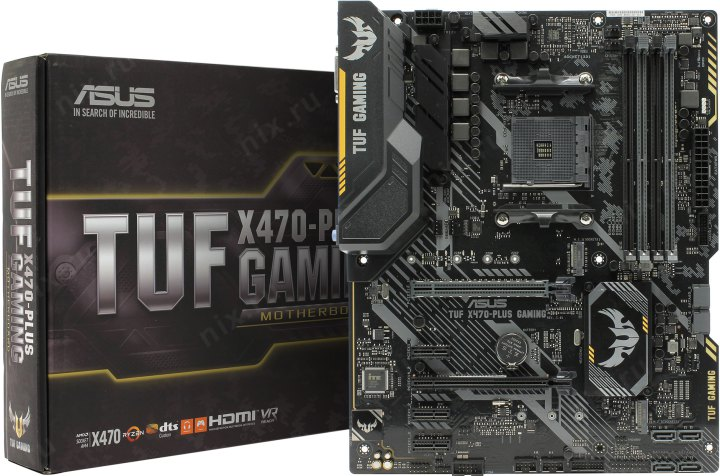
\includegraphics[scale=0.3]{motherboard.jpg} 
\end{figure}
\subsubsection{Характеристики}
\begin{table}[H]
    \centering
    \begin{tabular}{|l|l|}
    \hline
    Характеристика & Значение \\
    \hline
    Чипсет & 470x \\
    Сокет & AM4 \\
    Слоты расширения & 4xDDR4, 2x PCIe 16x, 3x PCI-E 2.0 \\
    Внешние порты & 1x DVI-D, 1x HDMI, 1x Type C, 2x USB 3.1, 2x USB 3.0, 2x USB 2.0\\
    Внутренние интерфейсы & 2x MKey SATA/PCI-E, 2x USB 3.0, 4x USB 2.0 \\
    Форм-фактор & ATX \\
    \hline
\end{tabular}
\end{table}
    
\subsection{Процессор}
Обоснование Ryzen дешевле аналогичного процессора Intel
\subsubsection{Фото}
\begin{figure}[H]
\centering
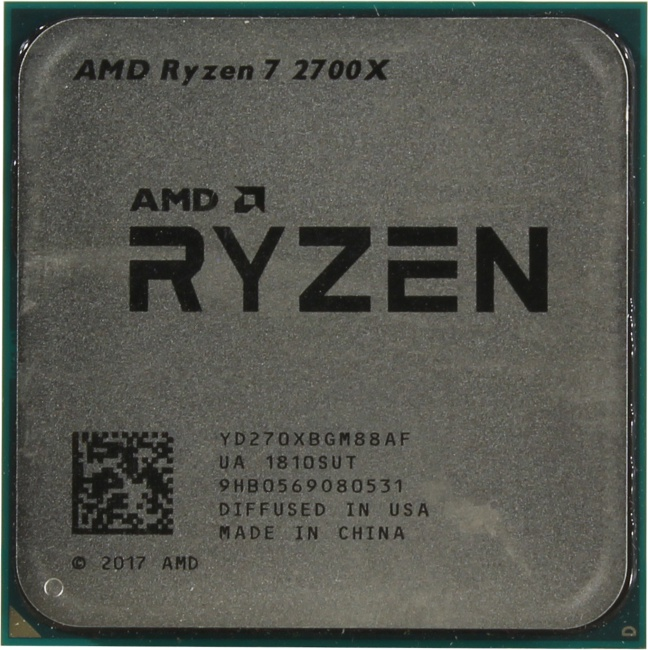
\includegraphics[scale=0.3]{cpu.jpg} 
\end{figure}

\subsubsection{Характеристики}
\begin{table}[H]
\centering
\begin{tabular}{|l|l|}
    \hline
    Характеристика & Значение \\
    \hline
    Тактовая частота & 3.7 Ghz (4.3 Ghz) \\
    Socket & AM4 \\ 
    Cache L1 & 96 Кб x8 \\
    Cache L2 & 512 Кб x8 \\
    Cache L3 & 8 Мб x2 \\
    \hline
\end{tabular}
\end{table}

\subsection{ОЗУ}
Обоснование: -
\subsubsection{Фото}
\begin{figure}[H]
\centering
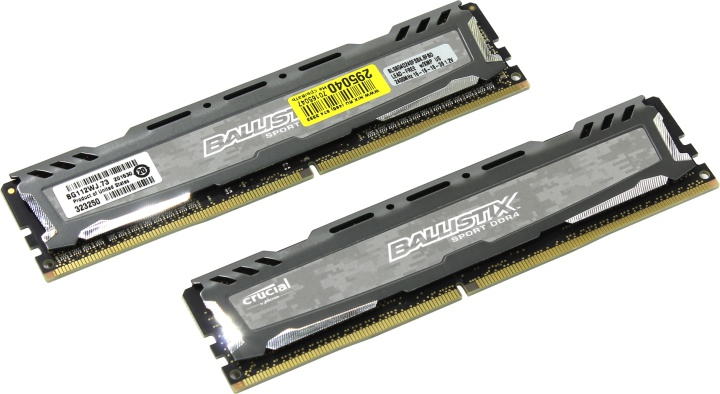
\includegraphics[scale=0.3]{ram.jpg} 
\end{figure}
\subsubsection{Характеристики}
\begin{table}[H]
    \centering
    \begin{tabular}{|l|l|}
    \hline
    Характеристика & Значение \\
    \hline
    Количество модулей & 2x \\
    Объем & 16 Gb \\
    Тип памяти & PC4-19200 (DDR4 2400 Mhz) \\
    \hline
\end{tabular}
\end{table}

\subsection{НЖМД}
Обоснование: -
\subsubsection{Фото}
\begin{figure}[H]
\centering
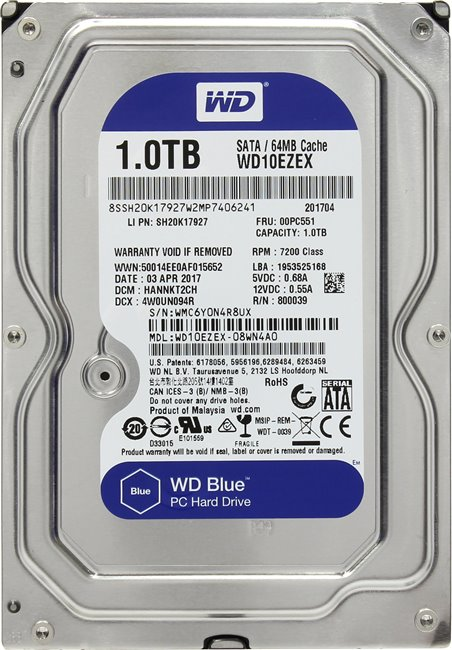
\includegraphics[scale=0.3]{harddrive.jpg} 
\end{figure}
\subsubsection{Характеристики}
\begin{table}[H]
    \centering
    \begin{tabular}{|l|l|}
    \hline
    Характеристика & Значение \\
    \hline
    Емкость накопителя & 1Tb \\
    Скорость вращения шпинделя & 7200Rpm \\
    Buffer size & 64Mb \\
    интерфейс & SATA III \\
    Форм-фактор & 3.5'' \\
    \hline
\end{tabular}
\end{table}

\subsection{Видеокарта}
Обоснование: нужна профессиональная видеокарта
\subsubsection{Фото}
\begin{figure}[H]
\centering
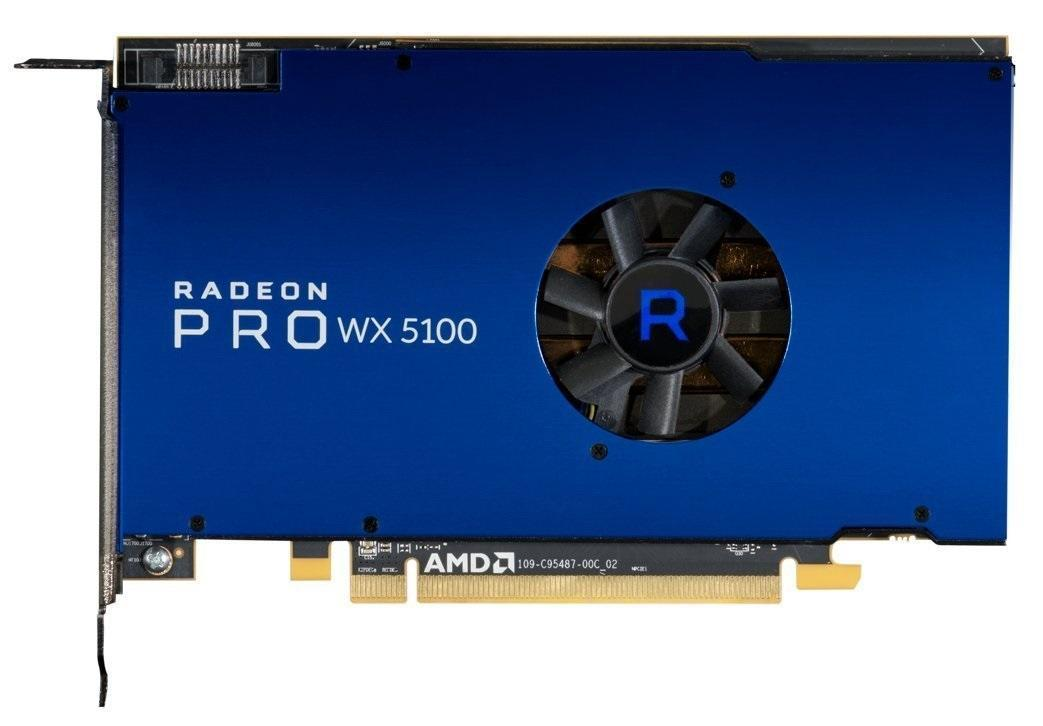
\includegraphics[scale=0.3]{gpu.jpg} 
\end{figure}
\subsubsection{Характеристики}
\begin{table}[H]
    \centering
    \begin{tabular}{|l|l|}
    \hline
    Характеристика & Значение \\
    \hline
    RAMDAC & 713 Mhz(1086 Mhz)\\
    Объем видеопамяти & 8 Gb \\
    Тип видеопамяти & GDDR5 \\
    Интерфейс & PCI-E \\
    Порты & 4x DisplayPort \\
    \hline
\end{tabular}
\end{table}

\subsection{Блок питания}
Обоснование: -
\subsubsection{Фото}
\begin{figure}[H]
\centering
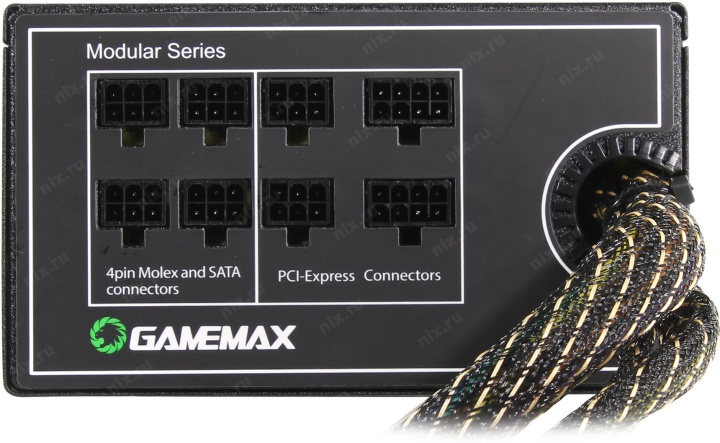
\includegraphics[scale=0.3]{power.jpg} 
\end{figure}
\subsubsection{Характеристики}
\begin{table}[H]
\centering
\begin{tabular}{|l|l|}
\hline
Характеристика & Значение \\
\hline
Форм-фактор & ATX \\
Входное напряжение & 100 ~ 240 В \\
Мощность & 	1050 W max. \\
Разъёмы & 24+8 pin, 24+4 pin, 20+4 pin, 4x 6/8-pin, 3x Molex, 9x SATA \\
\hline
\end{tabular} 
\end{table}

\subsection{Монитор}
Обоснование: широкий экран - хорошо для монтажа видео
\subsubsection{Фото}
\begin{figure}[H]
\centering
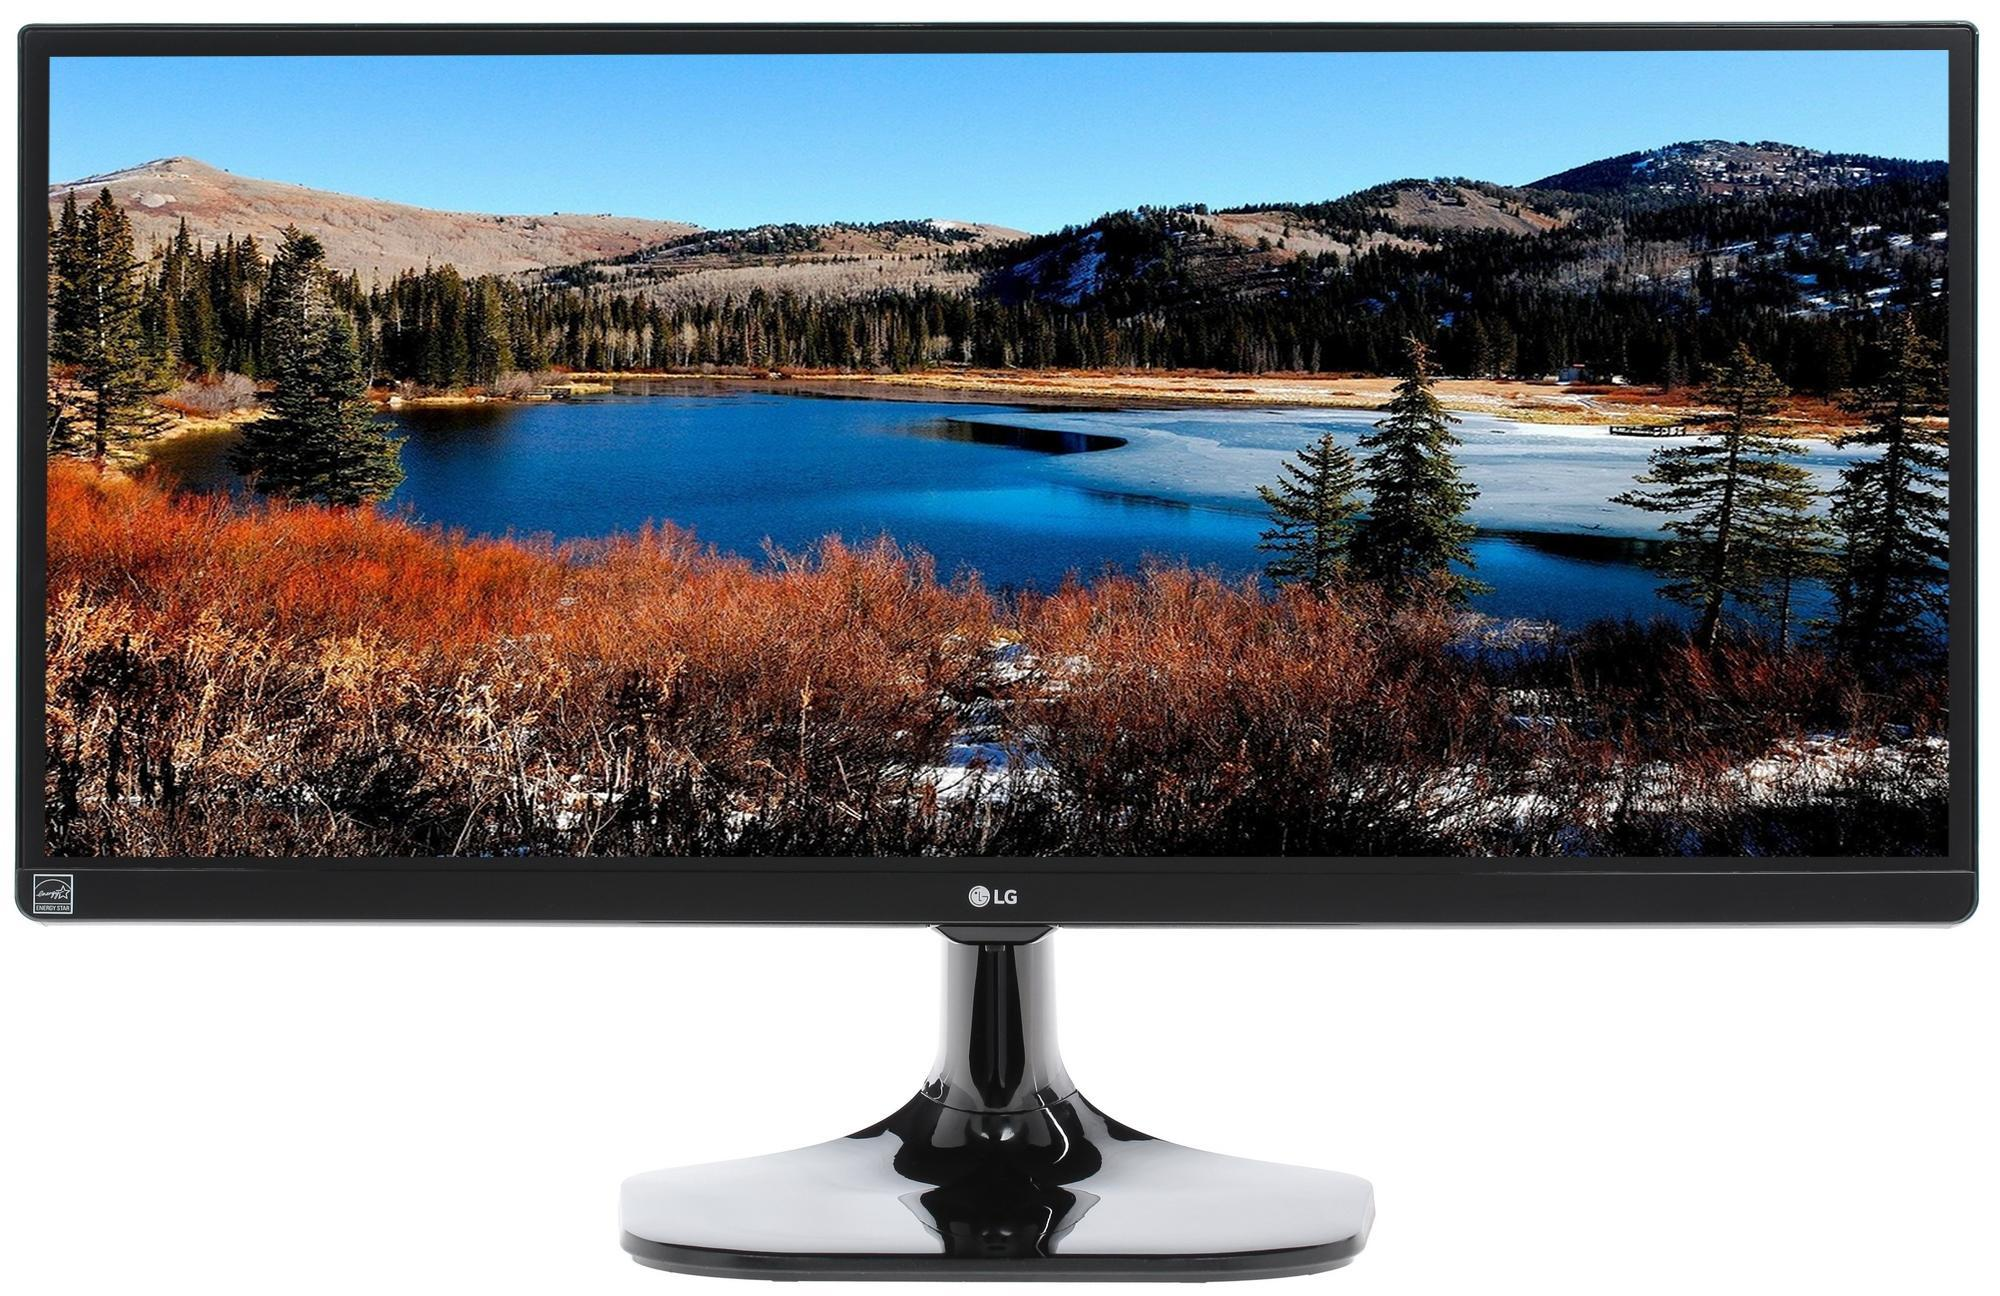
\includegraphics[scale=0.1]{mon.jpg} 
\end{figure}
\subsubsection{Характеристики}
\begin{table}[H]
\centering
\begin{tabular}{|l|l|}
\hline
Характеристика & Значение \\
\hline
Resolution & 2560x1080 \\
\hline
\end{tabular}
\end{table}


\section{Вывод}
В ходе лабораторной работы мы подготовили на заказ спецификацию компьютера для работы с видео

\end{document}